\begin{frame}{BGP communities}
    \begin{itemize}
    \item routes sent via BGP can have `communities'
    \item extra information tagged on routes sent via BGP
    \vspace{.5cm}
    \item large ISPs have lists of communities their customers/peers can use
    \item \ldots and these affect how those routes are used
    \end{itemize}
\end{frame}

\begin{frame}{aside: Internet2}
    \begin{itemize}
    \item non-profit networking consortium
    \item operations major US University-focused network
    \item basically one of UVa's ISPs
    \end{itemize}
\end{frame}

\begin{frame}{selected Internet2 BGP communities}
{\fontsize{9}{10}\selectfont\url{https://noc.net.internet2.edu/knowledge/policy-statements/internet2-bgp-communities.html}}
\begin{tikzpicture}
\node (a) {
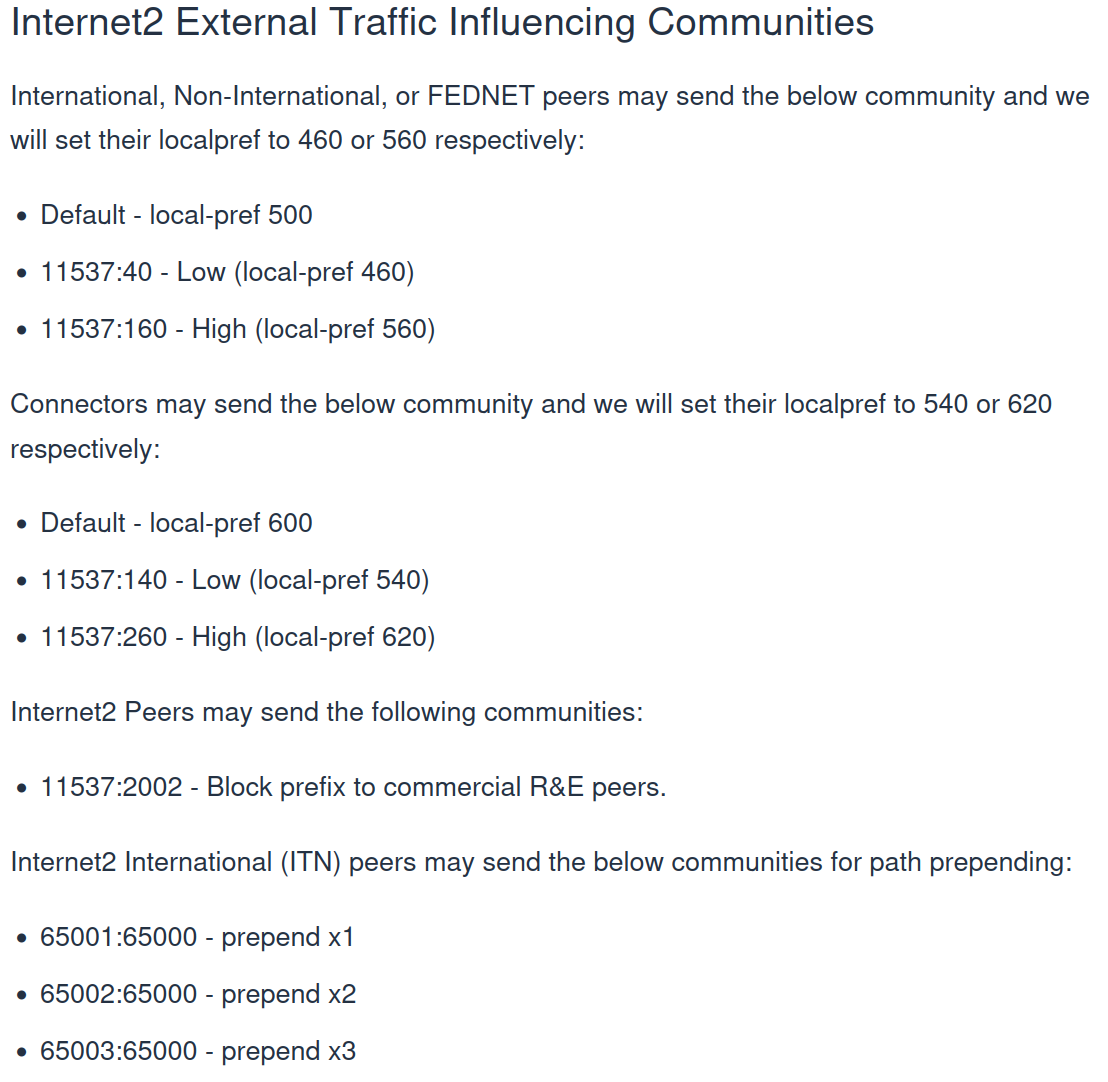
\includegraphics[width=0.49\textwidth]{../routing/i2-bgp-ext-comm}
};
\node[anchor=north west] (b) at (a.north east) {
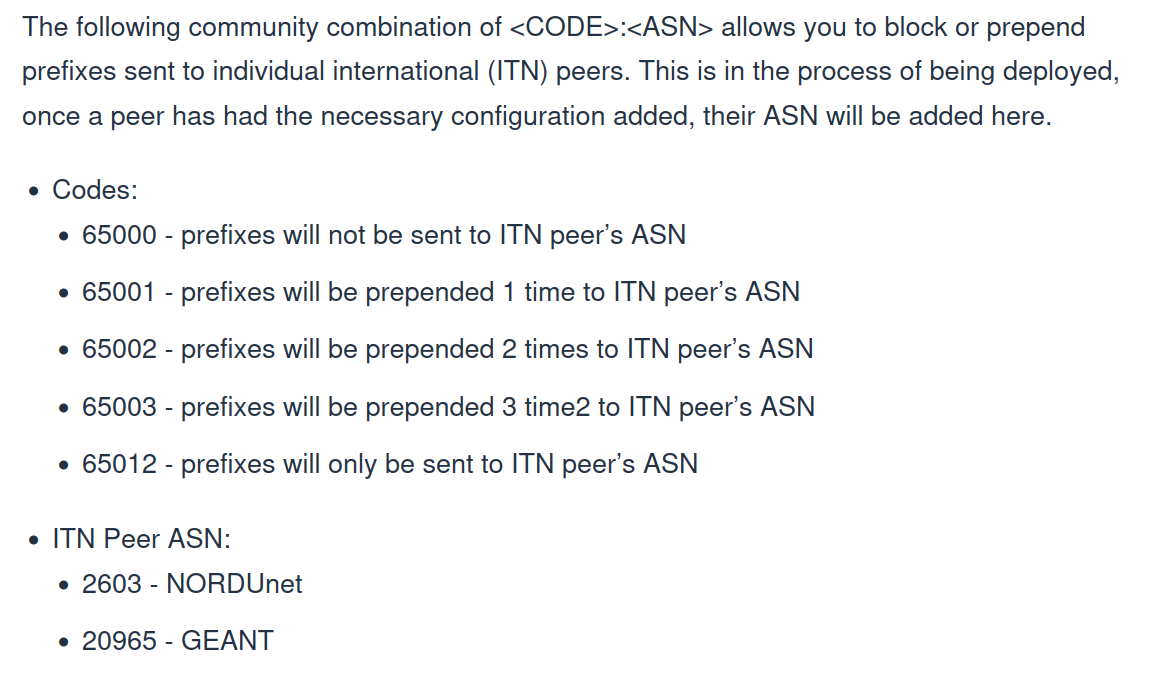
\includegraphics[width=0.39\textwidth]{../routing/i2-bgp-ext-comm2}
};
\node[anchor=north west] (c) at (b.south west) {
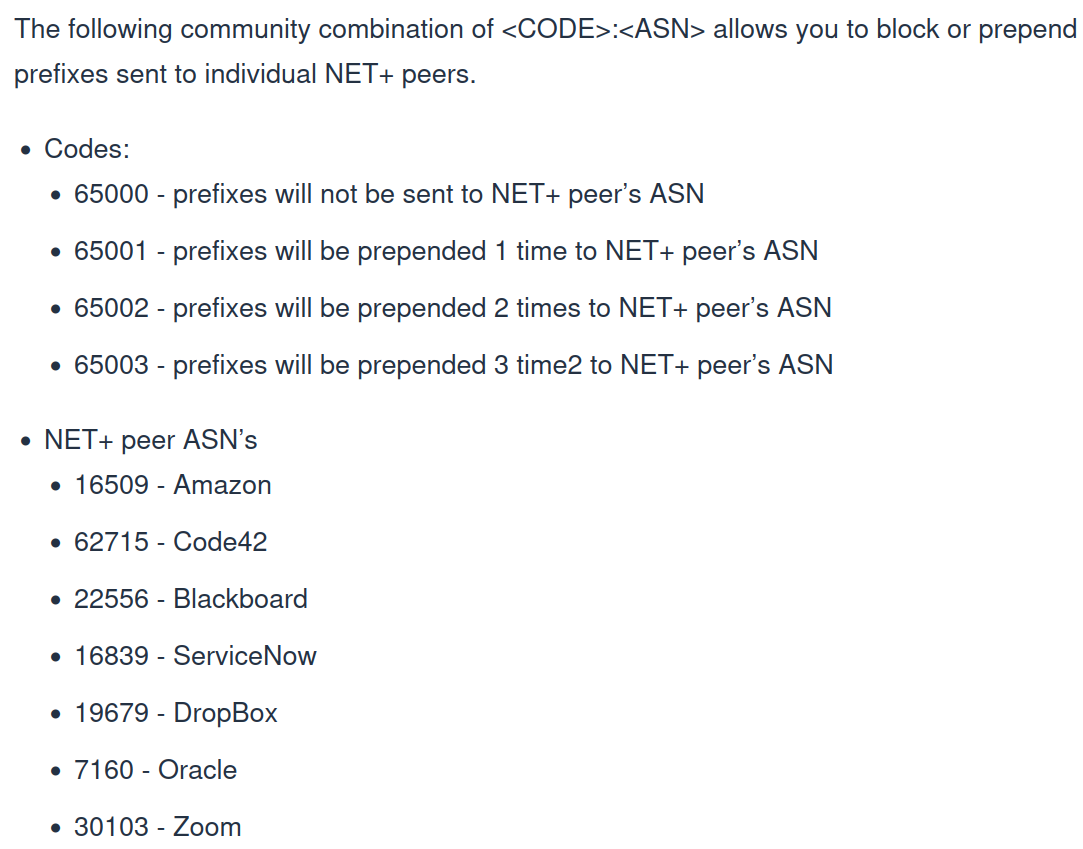
\includegraphics[width=0.39\textwidth]{../routing/i2-bgp-ext-comm3}
};
\end{tikzpicture}
\end{frame}

\begin{frame}{community options from prev slide}
\begin{itemize}
\item setting local-pref:
    \begin{itemize}
    \item you can decide how preferred your route is by Internet2
    \item maybe to make one primary, another secondary?
    \end{itemize}
\item blocking route from being sent to specific place
\item prepending Internet2's AS before forwarding prefix
    \begin{itemize}
    \item hopefully make that route less preferred by others
    \end{itemize}
\item prepending Internet2's AS before forwarding prefix to specific place
    \begin{itemize}
    \item hopefully make that route less preferred by that place
    \end{itemize}
\end{itemize}
\edn{frame}

\begin{frame}{other things with communities}
    \begin{itemize}
    \item Internet2 also uses communities to mark\ldots
    \item what location routes were learned from
    \item what type of organization routes were learned from
    \item whether Internet2 is only allowed to use the route non-commerically or not
    \item \ldots
    \end{itemize}
\end{frame}

